% Basic setup. Most papers should leave these options alone.
\documentclass[fleqn,usenatbib]{mnras}

% MNRAS is set in Times font. If you don't have this installed (most LaTeX
% installations will be fine) or prefer the old Computer Modern fonts, comment
% out the following line
%\usepackage{newtxtext,newtxmath}
% Depending on your LaTeX fonts installation, you might get better results with one of these:
\usepackage{mathptmx}
%\usepackage{txfonts}

% Use vector fonts, so it zooms properly in on-screen viewing software
% Don't change these lines unless you know what you are doing
\usepackage[T1]{fontenc}
\usepackage{ae,aecompl}

%%%%% AUTHORS - PLACE YOUR OWN PACKAGES HERE %%%%%

% Only include extra packages if you really need them. Common packages are:
\usepackage{savesym}
\usepackage{amsmath}
\savesymbol{iint}
\usepackage{txfonts}
\restoresymbol{TXF}{iint}

\usepackage{graphicx}	% Including figure files
\usepackage{amsmath}	% Advanced maths commands
\usepackage{amssymb}	% Extra maths symbols
\usepackage[ansinew]{inputenc}
\usepackage{amsfonts}
\usepackage{graphicx}
\usepackage{epsfig}
\usepackage{color}
\usepackage[normalem]{ulem}
\usepackage{natbib}
\usepackage{url}
%\usepackage{hyperref}
\usepackage{placeins}
\usepackage{caption}
\usepackage{subcaption}
\captionsetup{compatibility=false}

% By default the URLs are put in typewriter type in the body and the
% bibliography of the document when using the \url command.  If you are
% using many long URLs you may want to uncommennt the next line so they
% are typeset a little smaller.
%\renewcommand{\UrlFont}{\small\tt}

\def\aap{{A\&A}}
\def\AaA{{A\&A}}
\def\AJ{{AJ}}
\def\aj{{AJ}}
\def\ApJ{{ApJ}}
\def\apj{{ApJ}}
\def\apjl{{ApJL}}
\def\ApJL{{ApJL}}
\def\ApJSupp{{ApJS}}
\def\MN{{MNRAS}}
\def\mnras{{MNRAS}}
\def\mnrasl{{MNRAS Letters}}
\def\pasp{{PASP}}
\def\jcap{JCAP}
\def\pasj{{PASJ}}
\def\nat{Nature}
\def\ARAA{{ARA\&A}}
\def\apjs{{ApJS}}
\def\araa{{ARA\&A}}
\def\apss{{Ap\&SS}}
\def\cjaa{{ChJAA}}
\def\aaps{{A\&AS}}

\newcommand{\eg}{{e.g., }}
\newcommand{\ie}{{i.e., }}

% Use strikethrough and colors for revisions
\usepackage[normalem]{ulem}
\definecolor{gray}{rgb}{0.5,0.5,0.5}
\newcommand{\change}[1]{\textcolor{red}{#1}}

\pdfminorversion=5

\title[Star-galaxy Classification Using GANs]{Star-galaxy Classification Using Semi-Supervised Generative Adversarial Networks}

\author[E. J. Kim and R. J. Brunner]{
  Edward J.~Kim$^1$\thanks{jkim575@illinois.edu} and Robert J.~Brunner$^{2,3,4}$ \\
$^1$Department of Physics, University of Illinois, Urbana, IL 61801 USA\\
$^2$Department of Astronomy, University of Illinois, Urbana, IL 61801 USA\\
$^3$School of Information Sciences, University of Illinois, Champaign, IL 61820 USA\\
$^4$National Center for Supercomputing Applications, Urbana, IL 61801 USA\\
}

% These dates will be filled out by the publisher
\date{Accepted XXX. Received YYY; in original form ZZZ}

% Enter the current year, for the copyright statements etc.
\pubyear{2017}

% Don't change these lines
\begin{document}
\label{firstpage}
\pagerange{\pageref{firstpage}--\pageref{lastpage}}
\maketitle

\begin{abstract}
As current and forthcoming photometric surveys, such as the Dark Energy Survey (DES) and the Large Synoptic Survey Telescope (LSST),
probe large cosmological volumes, the majority of photometric observations are too faint for a uniform spectroscopic follow-up.
As a result, the number of unlabeled data available for training supervised machine learning algorithms will be orders of magnitude
greater than the number of labeled data.
Semi-supervised learning techniques are of great interest since they are able to capture the underlying data distribution
with only a small amount of labeled data.
We study the application of generative adversarial networks (GANs) to the star-galaxy classification problem
in a semi-supervised setting.
Using data from the Sloan Digital Sky Survey (SDSS), we demonstrate that semi-supervised GANs are able to produce
accurate and well-calibrated classifications using only a small amount of labeled examples.
We also show that the number count distributions of the images generated by GAN follow a similar distribution to
the SDSS photometric sample.
\end{abstract}

\begin{keywords}
methods: data analysis -- techniques: image processing -- methods: statistical
-- surveys -- stars: statistics -- galaxies:statistics.
\end{keywords}

% Introduction
\section{Introduction}
  \label{sec:introduction}

The Sloan Digital Sky Survey \citep[SDSS;][]{york2000sloan}, one of the most successful surveys to date,
has obtained photometric observations of more than $3 \times 10^8$ objects, covering more than one-third of
the sky.
The SDSS has also conducted spectroscopic follow-up observations of more than $3 \times 10^6$
objects \citep{eisenstein2011sdss}.
However, the spectroscopic sample is about one hundred times smaller than the photometric sample,
since spectroscopy is considerably more expensive than photometry in terms of telescope time.
Due to the difficulty of making spectroscopic measurements,
modern, large-scale surveys, such as the Dark Energy Survey (DES),
and the Large Synoptic Survey Telescope (LSST), are purely photometric surveys.
The scarcity of spectroscopic samples will only be exacerbated in the current and next generation of surveys,
as they probe larger cosmological volumes and the majority of photometric observations become too faint
for a spectroscopic follow-up.

Machine learning techniques have been a popular method for classifying stars and galaxies in large sky surveys.
\citet{odewahn1992automated} pioneered the use of artificial neural networks in star-galaxy classification.
Some of the more recent examples of applying machine learning techniques to the star-galaxy classification problem include
decision trees \citep[\eg][]{ball2006robust},
support vector machines \citep[\eg][]{fadely2012},
and convolutional neural networks \citep{kim2017star}.
All of these techniques are \emph{supervised} learning algorithms,
where the input attributes (\eg magnitudes or colors) are provided along with the truth labels (\eg star or galaxy).
We must be careful when extrapolating these supervised algorithms beyond the limits of the labeled data,
because most machine learning methods commonly assume that the labeled samples are governed by
the same or similar underlying data distribution as the target distribution where we apply our model to make predictions.

\emph{Semi-supervised learning} falls between supervised learning, where training data are completely labeled,
and unsupervised learning, where all training data are unlabeled,
Semi-supervised techniques make use of a large amount of unlabeled data, in conjunction with a small amount of labeled data,
to better capture the underlying data distribution.
Semi-supervised learning is of great interest because there will be many orders of magnitude
more unlabeled than labeled data available in future ground-based imaging surveys.

Generative adversarial networks (GANs) --- a class of state-of-the-art deep learning algorithms commonly used in
image-to-image translation applications --- are usually unsupervised,
but semi-supervised learning variants of GANs have recently been introduced
\citep{springenberg2016unsupervised,salimans2016improved,odena2016semi}.
Unsupervised GANs have previously been applied several astronomical applications,
but the main focus in these studies is image generation.
For example, using the COSMOS data, \citet{ravanbakhsh2017enabling} trained Variational Autoencoders,
another commonly used generative model, and GANs to generate new galaxy images
with the goal of synthesizing calibration sets for weak gravitational lensing.
\citet{mustafa2017creating} applied a GAN model to the problem of generating cosmological weak lensing convergence maps.
\citet{schawinski2017generative} showed that GANs are able to recover detailed features such as galaxy morphology
from artificially degraded images of low-redshift galaxies.

In this work, we study the application of GANs in generating realistic images of not only galaxies,
but also the stars and quasi-stellar objects (QSOs or quasars) in ground-based photometric surveys.
More importantly, we demonstrate that semi-supervised GANs are able to produce accurate and well-calibrated classifications
using only a small number of labeled examples.
The rest of the paper is organized as follows.
In Section \ref{sec:data}, we describe the SDSS data set and the image pre-processing steps.
In Section \ref{sec:methods}, we provide a brief overview of semi-supervised GANs.
In Section \ref{sec:results}, we present the main results of image generation and source classification using our semi-supervised GAN model.
Finally, we outline our conclusions in Section \ref{sec:conclusions}.

% Data
\section{Data}
  \label{sec:data}
  
%%%%%%%%%%%%%%%%%%%% POSTAGE STAMPS %%%%%%%%%%%%%%%%%%%% 

\begin{figure*}
  \centering
  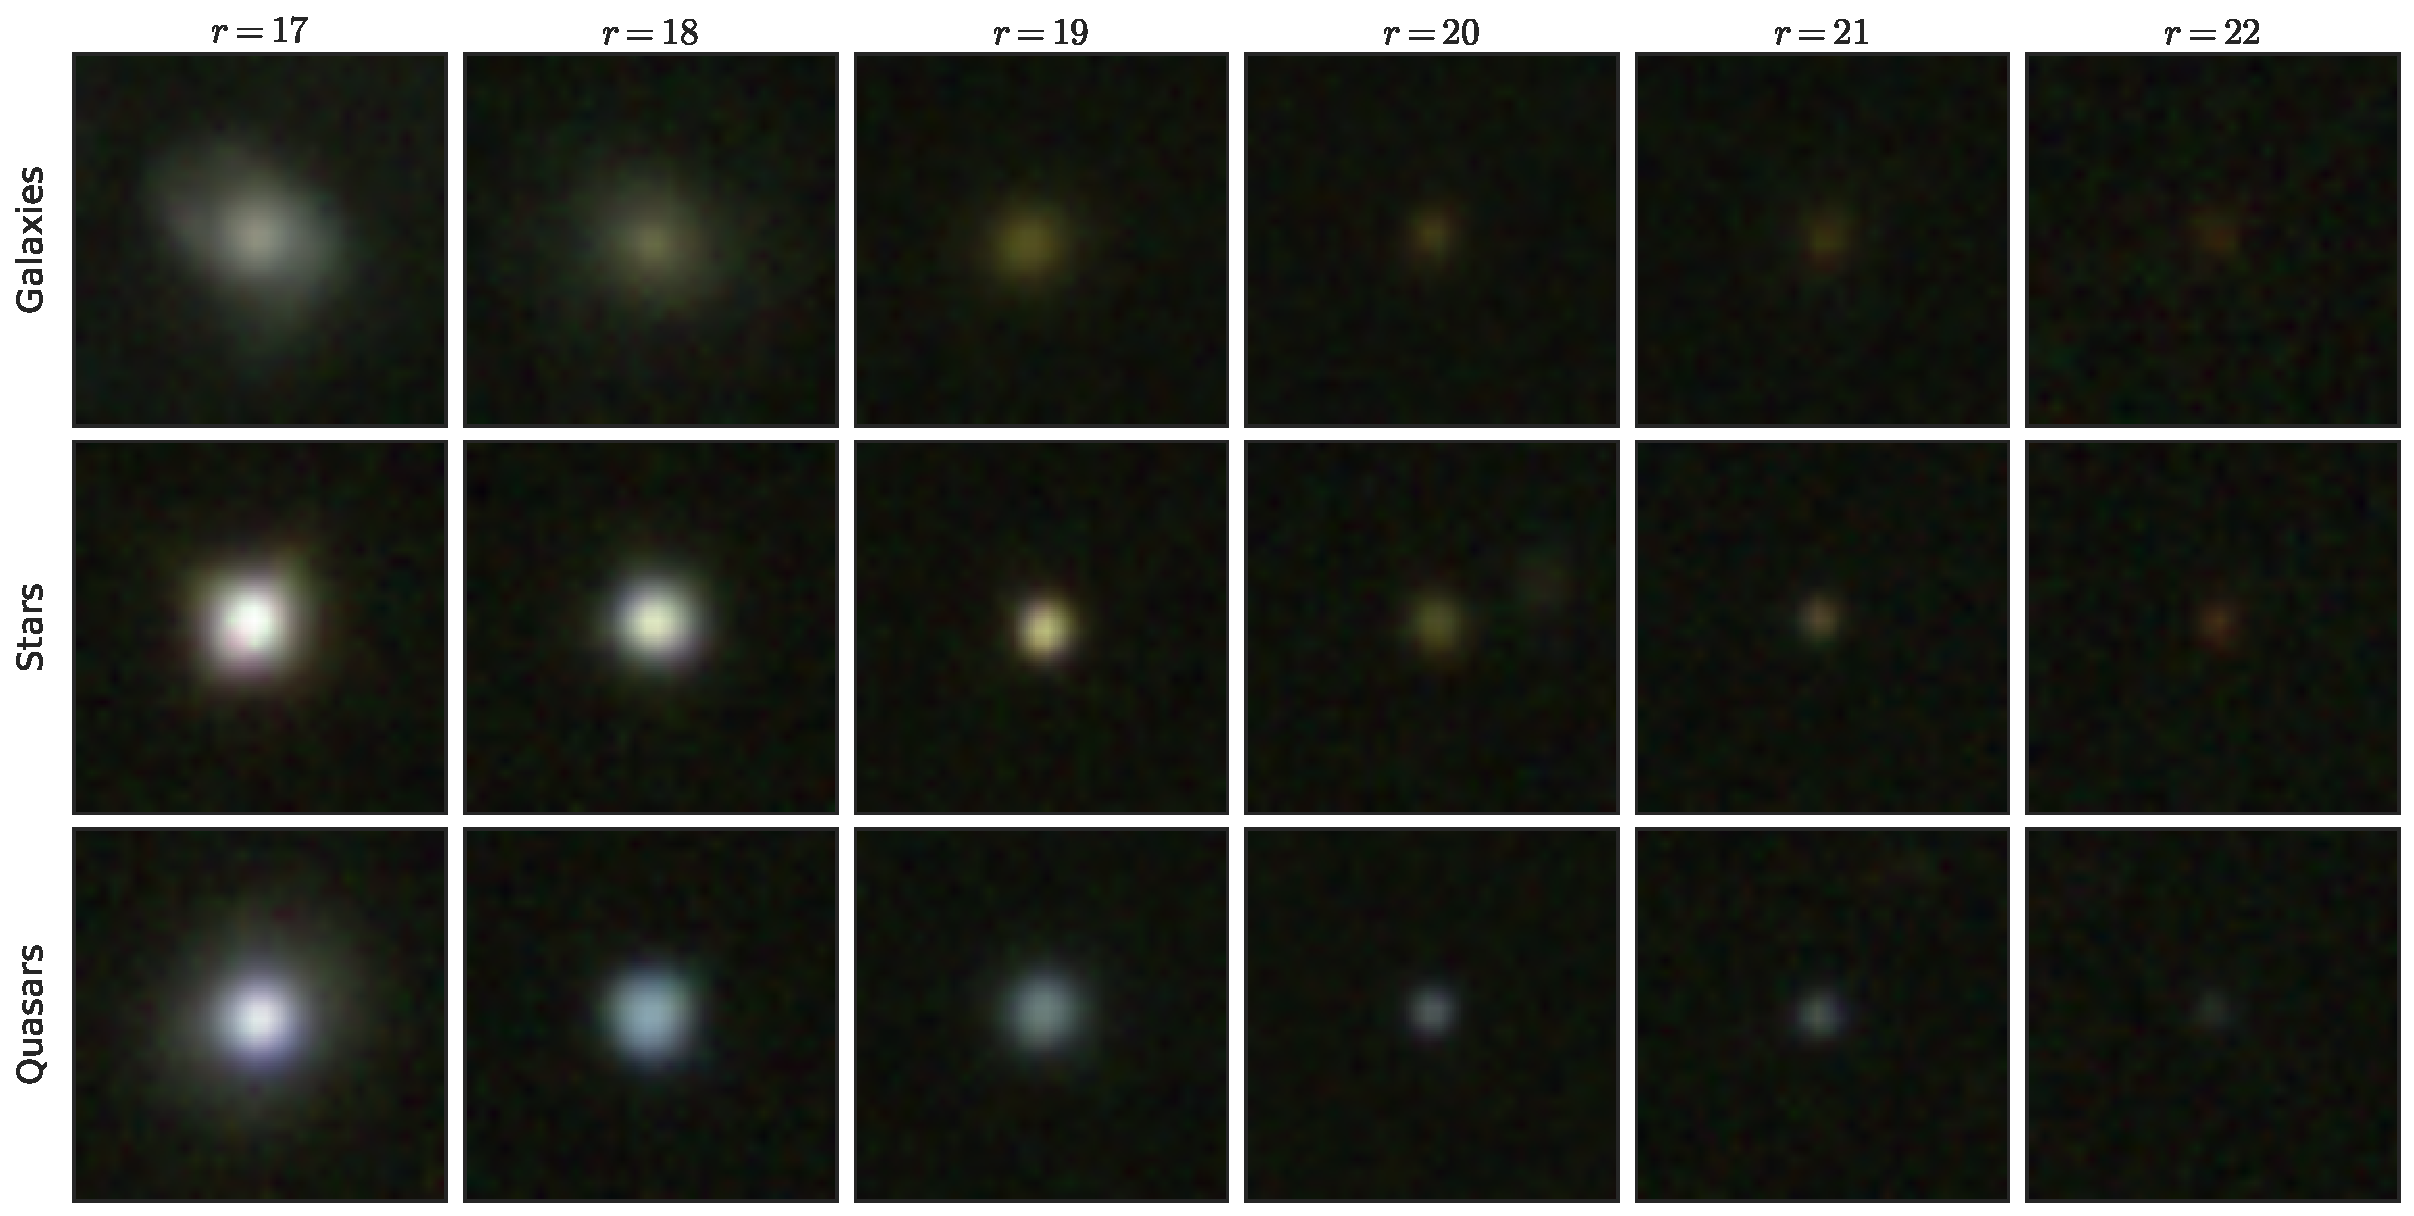
\includegraphics[width=\linewidth]{figures/sdss_stamps.pdf}
  \caption{
    Postage stamp images showing typical stars, galaxies, and quasars in SDSS as a function of $r$-band magnitude.
    The magnitude corresponds to \texttt{SExtractor}'s \texttt{MAG\_AUTO} (Kron-like elliptical aperature magnitude).
    Each image is $32 \times 32$ pixels and centered on the source of interest.
    The RGB image is created by mapping the R channel values to the $i$ band magnitude, G channel to $r$ band, and B to $g$ band.
    Each image is individually normalized for visualization purposes.
  }
  \label{fig:sdss_stamps}
\end{figure*}

\begin{figure*}
  \centering
  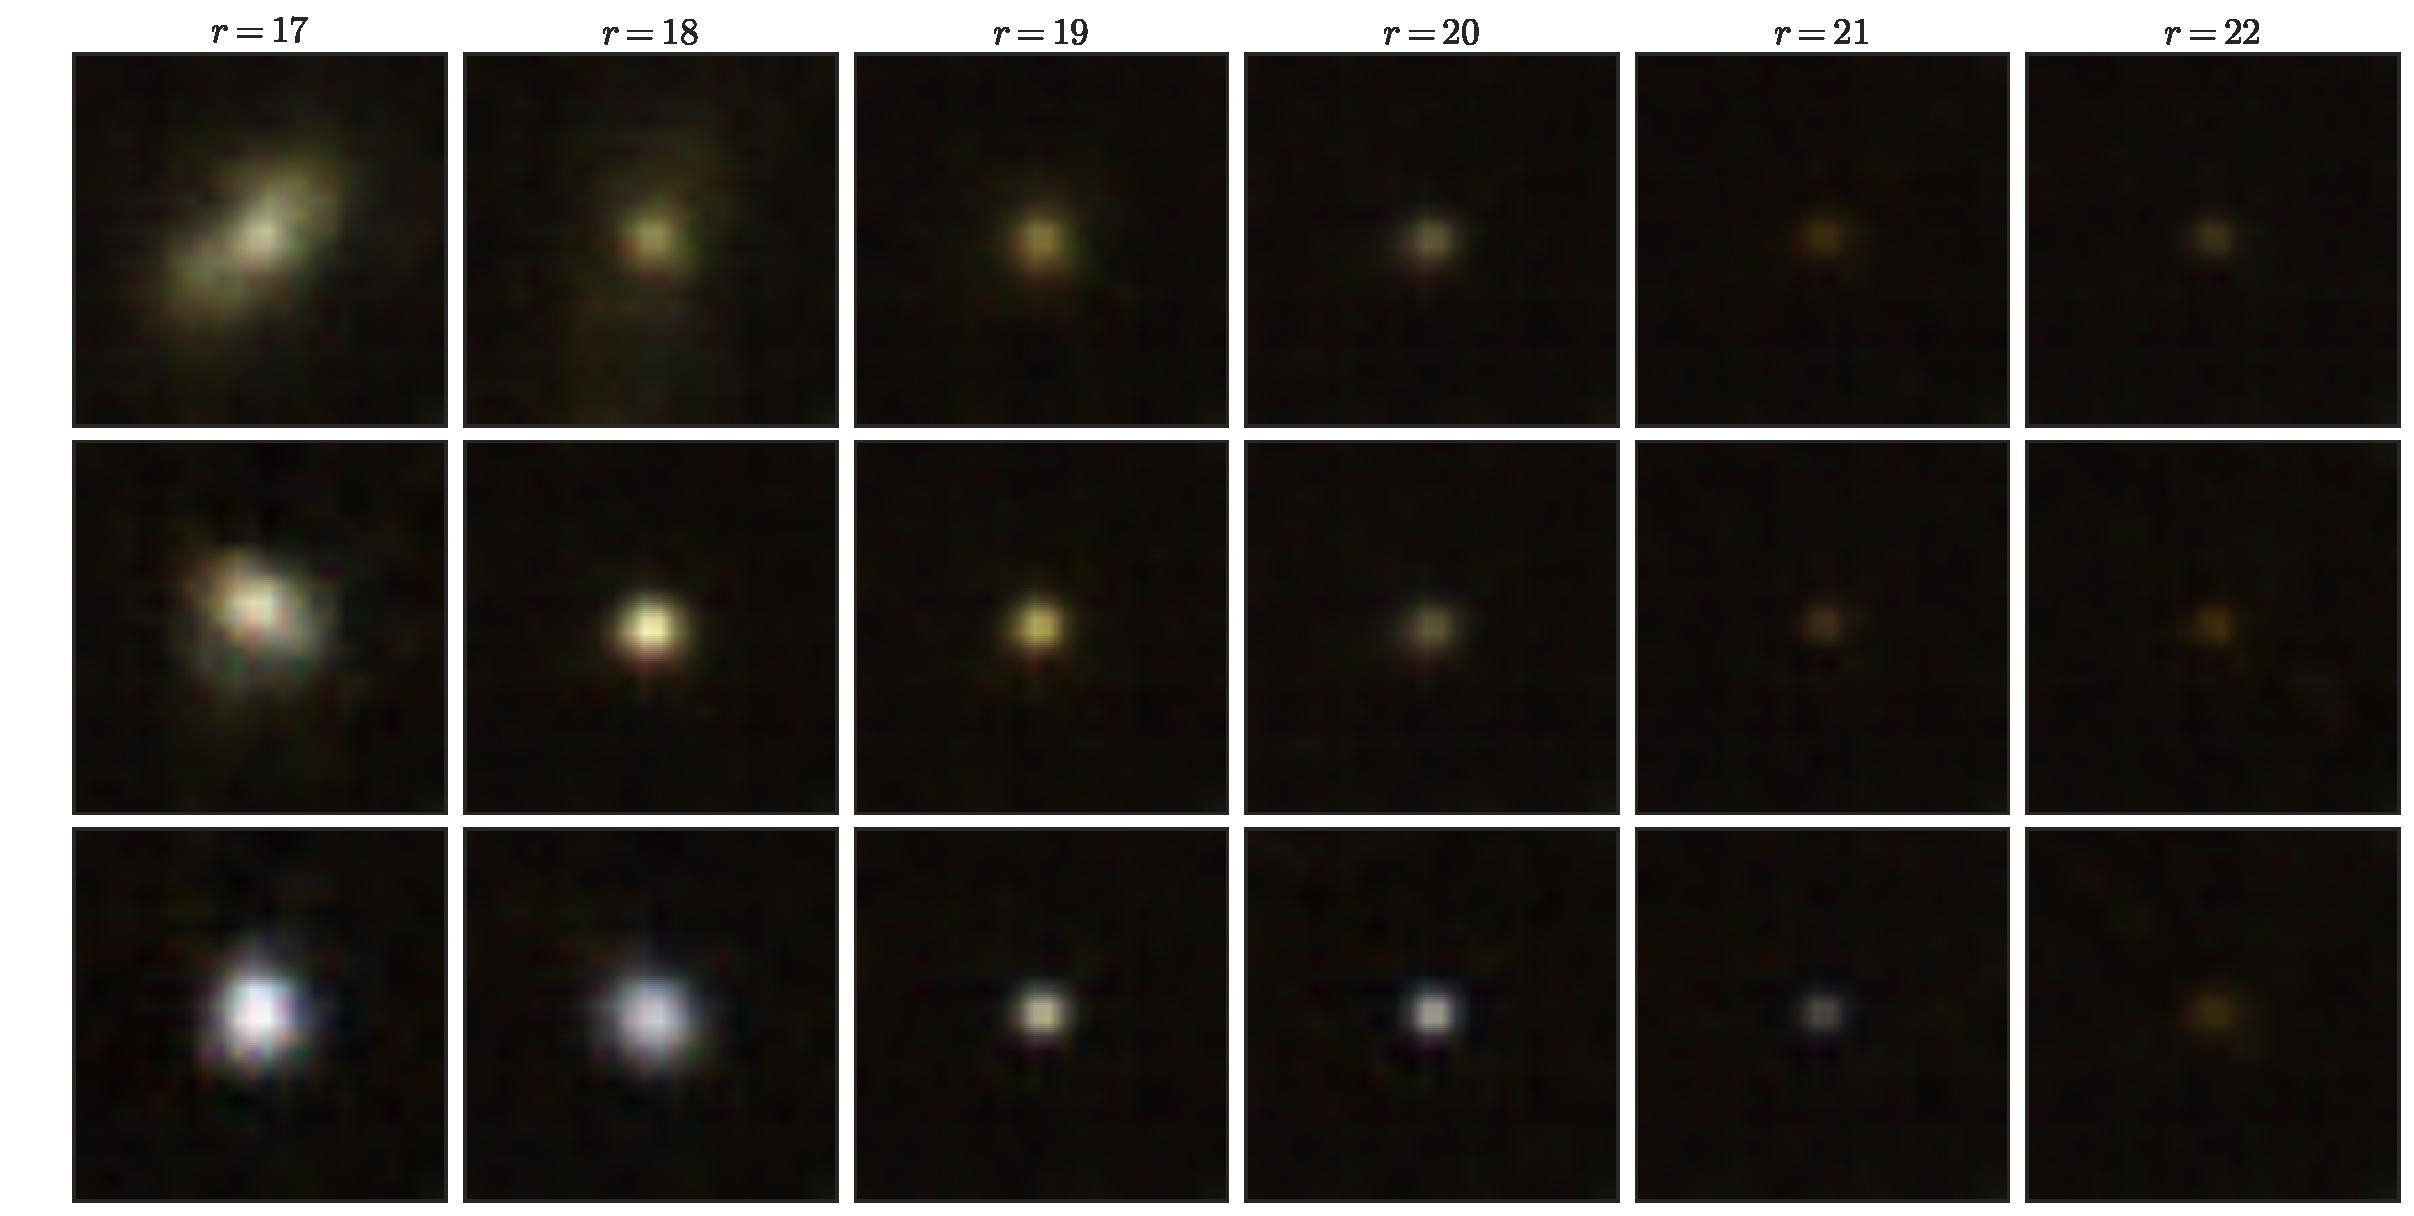
\includegraphics[width=\linewidth]{figures/gan_stamps.pdf}
  \caption{
    Sample $32 \times 32$ RGB images generated by our feature-matching GAN model as a function of $r$ band magnitude.
    Although the generated images for bright objects are slightly blurry and lack some details,
    the model generated, faint objects appear indistinguishable from real, faint objects.
    Since most objects are faint, the magnitude and half-light radius statistics of GAN generated images are in good agreement
    with the SDSS distribution as shown in Section \ref{sec:image_stats}.
    }
  \label{fig:gan_stamps}
\end{figure*}

%%%%%%%%%%%%%%%%%%%%

  
To demonstrate the performance of our approach, we follow a similar approach to our previous 
work \citep{kim2017star}.
However, we restrict our analysis to data from the SDSS survey in this paper.
We use SDSS because of the the large number of objects and the concurrent spectroscopy.
In this section, we briefly describe the SDSS data set and the image pre-processing steps for
preparing training examples.

The SDSS survey, one of the largest astronomical surveys that has ever existed,
covers 14,555 square degrees in five bands: $u$, $g$, $r$, $i$, and $z$.
The twelfth data release \citep{alam2015eleventh}, the final data release from SDSS phases I--III,
contains photometry of over $3 \times 10^8$ objects with a limiting magnitude of $r \approx 22$.
More than $3 \times 10^6$ objects from the photometric catalog were also targeted for spectroscopy \citep{eisenstein2011sdss}.

In a semi-supervised learning setting, we typically have a large amount of unlabeled data
and a small amount of labeled data.
Thus, the data sets we use in this work consists of an \emph{unlabeled} training set,
a \emph{labeled} training set, and a blind, \emph{labeled} test set.
For the unlabeled training set, we use the \texttt{photoObj} view of the publicly available CasJobs server \footnote{\url{http://skyserver.sdss.org/casjobs/}} \citep{li2008casjobs},
and randomly select $1 \times 10^6$ objects.
We exclude objects with bad photometric observations as follows.
We only include objects with magnitudes between 0 and 40;
we consider only objects with the half-light radius (as measured by the exponential and de Vaucouleurs light profiles)
in the $r$ band less than 30 arc seconds;
we also exclude any objects with warning flags in the photometric measurement;
and we exclude any images with missing or masked values.
After using the CasJobs server to select objects with clean photometry,
we download the FITS images for SDSS fields covering these objects.
Using the astrometry information in the FITS headers and the \texttt{Montage} \footnote{\url{http://montage.ipac.caltech.edu/}} software,
we align each image in $u$, $g$, $i$, and $z$ bands to the $r$-band image.
To generate cutout images of size $32 \times 32$ pixels that can be used as input to our GAN framework,
we use \texttt{SExtractor} to center each object in the cutout image.
Furthermore, we convert all flux values in the FITS files to luptitudes
\citep[\ie inverse hyperbolic sine magnitudes;][]{lupton1999modified}.
Finally, we use the dust reddening map of \citet{schlegel1998maps} to account for extinction.
Sample postage stamps of typical galaxies, stars, and quasars are shown in Figure \ref{fig:sdss_stamps}.

The labeled training sets and the test set are drawn from objects in the \texttt{specObj} view of the DR12 catalog.
We randomly select a total of $1 \times 10^6$ sources from \texttt{SpecObj}, and follow the same image pre-processing steps.
In addition to removing bad photometry similarly to the unlabeled data,
we exclude some bad spectroscopic observations by only including objects with no warning flags in the spectroscopic measurement
(\ie \texttt{zWarning = 0})
and sources with the spectroscopic redshift less than 2 or its error less than 0.1.
We randomly split the labeled objects into a blind test set of size $ 2 \times 10^5$ and multiple labeled training sets
with only a small number of labeled data in each set for running multiple experiments (See Section \ref{sec:classification}).
To optimize the model, we perform eightfold cross-validation on the labeled training set.

We emphasize that this setup is considerably different from a typical training-test split used in a supervised setting.
In a supervised setting, the learning algorithm would be trained on the SDSS spectroscopic sample
although it would eventually have to be applied to the SDSS photometric sample.
As shown in Figure \ref{fig:spec_phot}, the SDSS photometric sample is considerably fainter than the SDSS spectroscopic sample,
and they have different distributions due to the target selection process.
This can become a major drawback of any supervised algorithms since most machine learning algorithms assume that both
training and test sets are drawn from the same parent distribution,
However, in our semi-supervised setting, only a small number of labeled data are used for training,
and the vast majority of training data are drawn from the SDSS photometric sample.
As discussed in the following sections, this could be an advantage for semi-supervised learning because
it will not only require a smaller number of labeled examples to obtain a comparable performance
but also will extrapolate better beyond the limits of the training data.

%%%%%%%%%%%%%%%%%%%% Phot Spec Distribution %%%%%%%%%%%%%%%%%%%% 

\begin{figure}
  \centering
  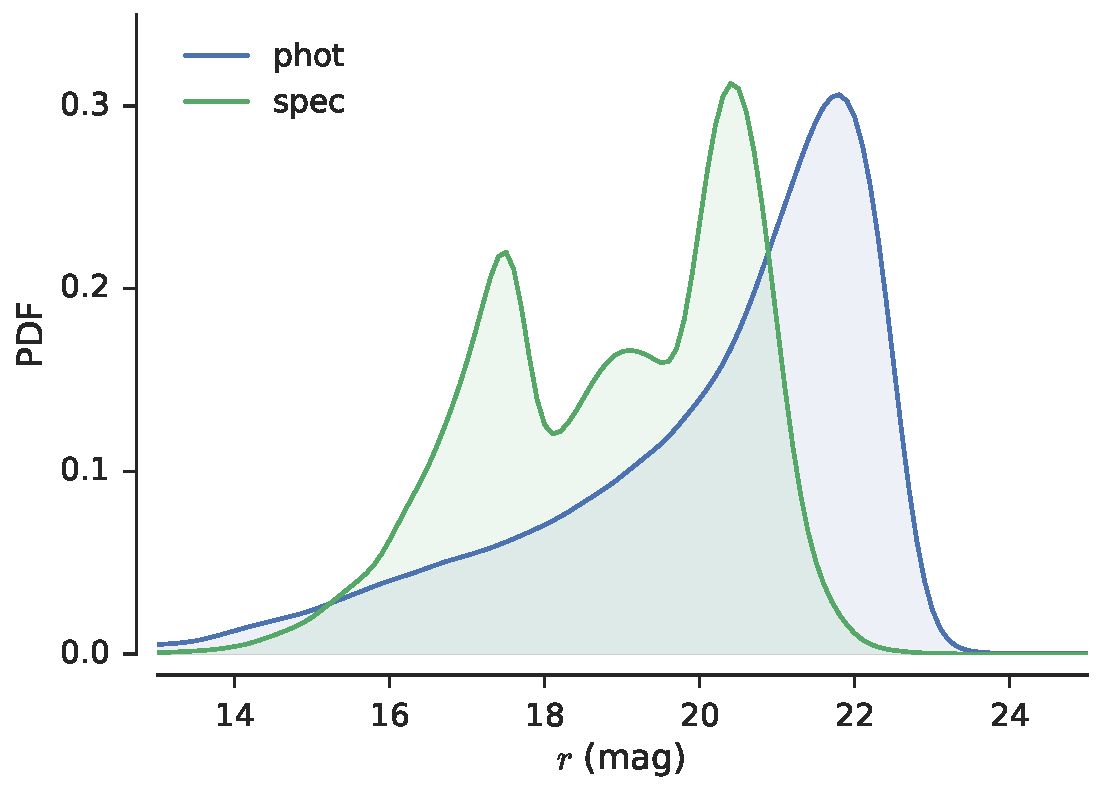
\includegraphics[width=\columnwidth]{figures/spec_phot.pdf}
  \caption{
    Number counts of SDSS objects as a function of the $r$-band magnitude as estimated by kernel density estimation (KDE).
    The blue curve shows the KDE of $1 \times 10^6$ objects in the unlabeled training set,
    which were randomly selected from the \texttt{PhotoObj} view.
    The green curve is the KDE of $2 \times 10^5$ objects in the labeled test set,
    which were randomly selected from the \texttt{SpecObj} view.
    We use the SDSS \texttt{cModelMag}, the composite model magnitude resulting from the best-fitting linear combination
    of the best-fit exponential and de Vaucouleurs fits.
    All KDEs presented here and throughout this paper use a Guassian kernel and Silverman's rule to determine
    the kernel bandwidth \citep{silverman1986density}.
  }
  \label{fig:spec_phot}
\end{figure}

%%%%%%%%%%%%%%%%%%%%

% Generative Adversarial Networks
\section{Methods}
  \label{sec:methods}
  
Generative adversarial networks \citep[GANs;][]{goodfellow2014generative} are a class of methods where
a generative model is pitted against a discriminative model.
In this section, we briefly introduce the standard, unsupervised GAN, and describe how we can perform semi-supervised learning
by replacing the discriminator in conventional GANs with a classifier.
We also briefly present how uncertainty analysis of model predictions can be performed in deep learning.
For more details, interested readers are referred to the references herein.

\subsection{Semi-Supervised Generative Adversarial Networks}

In most GANs, the generator network $G$ takes random noise $p_z \left( z \right)$
as input and produces samples $x$ from the data distribution $p \left( x \right)$.
The discriminator network $D$ is then trained to classify real data and fake samples
from the generator $G$.
In the adversarial setting, the generator is trained to fool the discriminator into classifying its
fake instances as real.
In other words, we train $D$ to maximize $D \left( x \right)$,
the probability of classifying real training examples as real,
and maximize $\log \left( 1 - D \left( G \left( z \right) \right) \right)$,
the probability of classifying samples from $G$ as fake.
In the original GAN framework of \citet{goodfellow2014generative}, the loss function for training $D$ is
\begin{equation}
  L = - \mathbb{E}_{x \sim p} \log D \left( x \right)
      - \mathbb{E}_{z \sim p_z} \log \left( 1 - D \left( G \left( z \right) \right) \right),
  \label{eq:original_gan_loss}
\end{equation}
and $G$ is trained to minimize $\log \left( 1 - D \left( G \left( z \right) \right) \right)$.
When the generator and the discriminator are trained alternatively to converge to a fixed point,
the fake samples generated by $G$ are realistic enough to fool the discriminator.

Traditionally, the discriminator network in a normal GAN employs a binary classification,
but it can also be implemented with any standard classifier that classifies the input $x$
into one of $K$ possible classes~\citep{salimans2016improved, odena2016semi}.
In this modified setting, we increase the number of output classes in our classifier from $K$ to $K+1$,
where real data are classified into the first $K$ classes and samples from the GAN generator $G$ are
classified into the new $\left( K + 1 \right)$-th class.
We now have a semi-supervised classifier, since we can use unlabeled data to maximize
$P_{\mathrm{C}} \left( y \leq K \mid x \right)$,
the probability that the classifier $\mathrm{C}$ classifies input into one of the $K$ classes.
Our loss function for training $C$ becomes
\begin{align}
  L &= L_{\text{supervised}} + L_{\text{unsupervised}}
    \label{eq:total_loss} \\
  L_{\text{supervised}} &= -\mathbb{E}_{x, y \sim p} \log P_{\mathrm{C}} \left( y \mid x, y \leq K \right)
    \label{eq:supervised_loss} \\
  L_{\text{unsupervised}} &= - \mathbb{E}_{x \sim p} \log P_{\mathrm{C}} \left( y \leq K \mid x \right) \nonumber \\
    & \quad - \mathbb{E}_{x \sim p_z} \log P_{\mathrm{C}} \left( y = K + 1 \mid x = G \left( z \right) \right).
    \label{eq:unsupervised_loss}
\end{align}
Note we that recover Equation \ref{eq:original_gan_loss} when we substitute
$P_{\mathrm{C}} \left ( y = K + 1 \mid x \right) = 1 - D(x)$ or
$P_{\mathrm{C}} \left( y \leq K \mid x \right) = D(x)$ into Equation \ref{eq:unsupervised_loss},
and our unsupervised loss function $L_{\text{unsupervised}}$ is therefore equivalent to the original GAN objective.

We also use \textit{feature matching}, one of the techniques proposed by \citet{salimans2016improved} to address
the instability of GANs.
A major hurdle in training GANs is mode collapse, where the generator overtrains on the current discriminator
and fake samples from the generator capture only a few of modes from the data.
In feature matching GANs, the objective of the generator is to match the statistics between the generator distribution
and the real distribution rather than minimize $\log \left( 1 - D \left( G \left( z \right) \right) \right)$.
Specifically, we train $G$ to minimize
$ \big\lVert \mathbb{E}_{x \sim p} f \left( x \right) - \mathbb{E}_{z \sim p_z} f \left( G \left( z \right) \right) \big\rVert^2_2$,
where $f(x)$ denote the features (\ie activations) on the final intermediate layer before the fully-connected layer.

Following \cite{salimans2016improved}, we use deconvolutional layers, batch normalization, weight normalization~\citep{salimans2016weight},
and leaky ReLU activation functions in our generator network.
For optimization, we use Adam optimizer with exponential decay rate of 0.5 for the first moment estimates.
Our discriminator network consists of seven convolutional layers, two network-in-network layers~\citep{lin2013network}, one global pooling layer,
and a fully connected layer.
We also use dropout, weight normalization, leaky ReLU activation functions, and Adam optimizer in our discriminator.

\subsection{Dropout Sampling}
  \label{sec:dropout_sampling}
 
To obtain predictive probabilities, standard deep learning techniques use the softmax function
at the end of the pipeline.
However, using the softmax output does not adequately address model uncertainty,
because most algorithms pass the predictive mean through the softmax rather than
the entire probability distribution.
\citet{gal2016dropout} have recently shown that model uncertainty
can be obtained from deep neural networks that use a technique called dropout.
Dropout is a technique used to avoid overfitting, and it consists of
randomly setting to zero the output of each hidden neuron of the previous layer with some probability.
Since a neuron can be removed at any time, it cannot rely on the presence of other neurons
in the same layer and is forced to learn more robust features.
Dropout has been a ubiquitous technique in deep learning since \citet{hinton2012improving}
proposed it as a way to avoid overfitting, but most deep learning practitioners
do not utilize the information contained in the dropout layers.
To estimate the predictive mean and predictive uncertainty,
we simply collect Monte Carlo samples from the networks and then compute
the standard deviation over the softmax outputs of the samples.
This adds almost no additional computational cost at training time and often improves predictive performance.
%Furthermore, the model uncertainty enables a user to obtain a pure sample for population studies,
%or to optimize the allocation of observing time by selecting objects for follow-up spectroscopy.

% Results
\section{Results}
  \label{sec:results}

In this section, we first evaluate the quality of generated images by comparing the magnitude and size distributions
between real and generated images.
We then present the classification performance of our semi-supervised GAN model on the SDSS data set.
We also demonstrate that dropout sampling not only improves the performance but also enables us to obtain the model uncertainty.

\subsection{Image Statistics}
  \label{sec:image_stats}


\begin{figure}
  \centering
  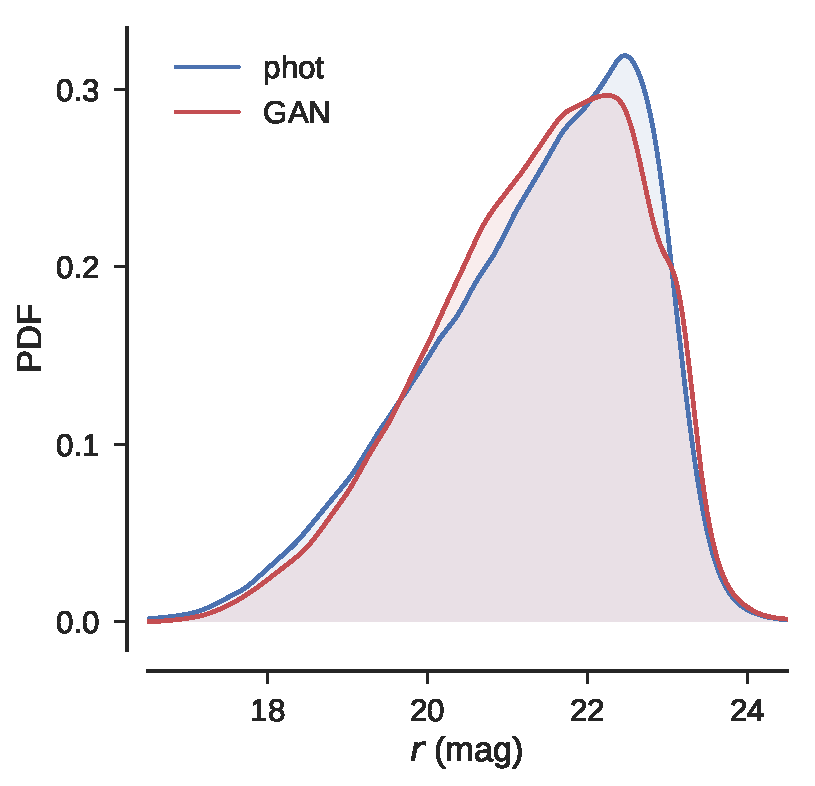
\includegraphics[width=\columnwidth]{figures/mag_kde.pdf}
  \caption{
      Comparison of $r$-band magnitude distributions between real SDSS images and GAN generated images.
      The blue curve shows the KDE of $1 \times 10^5$ objects in the unlabeled training set.
      The red curve shows the KDE of $1 \times 10^5$ objects generated by GAN.
      We use the \texttt{SExtractor}'s \texttt{MAG\_AUTO} values as an approximate total magnitude for each objects.
      }
  \label{fig:mag_kde}
\end{figure}

\begin{figure}
  \centering
  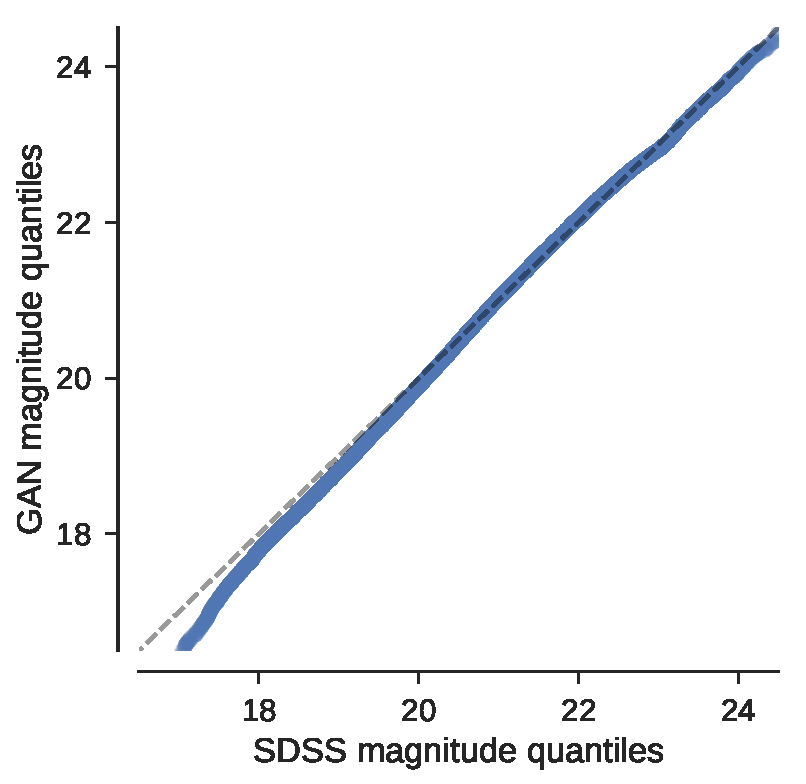
\includegraphics[width=\columnwidth]{figures/mag_qq.pdf}
  \caption{Q-Q plot comparing the distributions of $r$-band magnitudes between real SDSS images and GAN generated images.}
  \label{fig:mag_qq}
\end{figure}

\begin{figure}
  \centering
  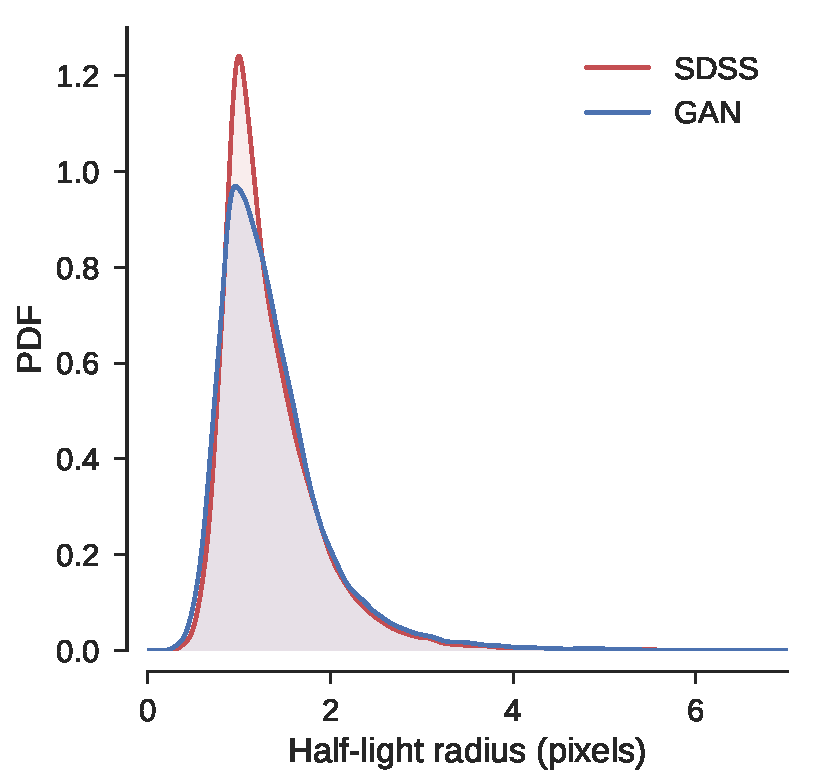
\includegraphics[width=\columnwidth]{figures/size_kde.pdf}
  \caption{Comparison of half-light radius distributions between real SDSS images and GAN generated images.}
  \label{fig:size_kde}
\end{figure}

\begin{figure}
  \centering
  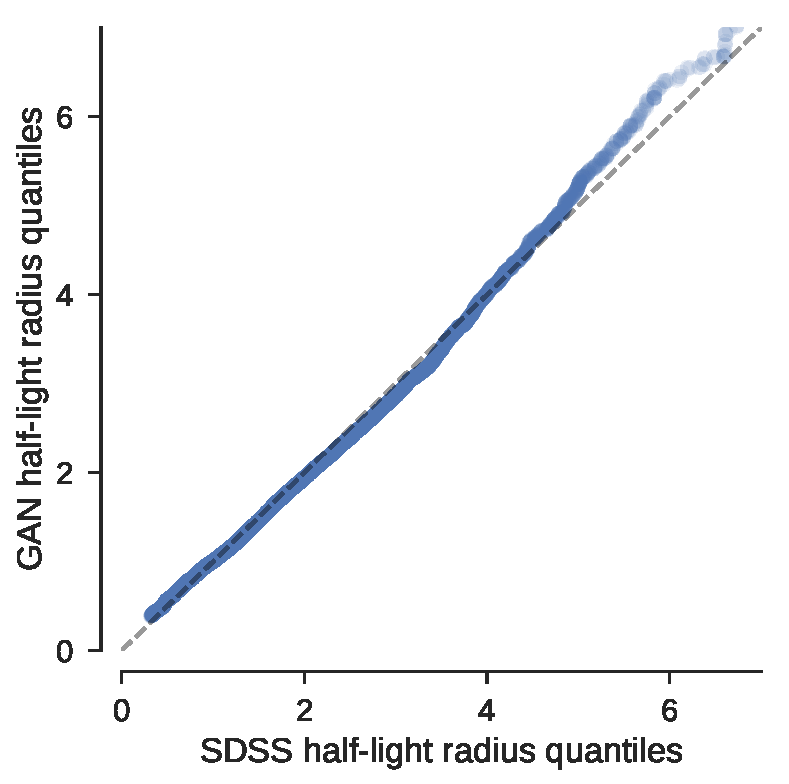
\includegraphics[width=\columnwidth]{figures/size_qq.pdf}
  \caption{Q-Q plot comparing the distributions of half-light radius between real SDSS images and GAN generated images.}
  \label{fig:size_qq}
\end{figure}

By using GANs for semi-supervised learning, we have an added benefit of being able to synthesize
new images of stars, galaxies, and quasars.
Samples of generated images for different magnitude ranges are shown in Figure \ref{fig:gan_stamps}.
Comparing the generated images to Figure \ref{fig:sdss_stamps}, the bright objects in GAN generated images are
slightly blurry and lack fine details, while the faint objects appear similar to the real SDSS images.

Generative models could potentially be an inexpensive alternative to
image simulation pipelines, such as the \textit{GalSim} package \citep{rowe2015galsim},
which require high-quality images with high resolution and signal-to-noise ratio
as input to the pipeline.
However, it is important to evaluate the goodness-of-fit in order to use generative models
in practical applications.
The evaluation of generative models is still an active area of research \citep{theis2016note}.
In the deep learning community, where the focus is on natural images,
many researchers rely on visual inspection to assess the quality of images generated by GANs.
In the case of scientific applications of generative models, however,
we can also assess the quality of the generated images by studying the characteristic image statistics.

The most relevant image statistics for star-galaxy classification are the magnitude and size (\ie half-light radius) distributions.
Figure \ref{fig:mag_kde} compares the $r$-band magnitude distribution of generated images to that of the SDSS photometric sample.
To compare the two probability distributions, we also generate a quantile-quantile plot
\citep[Q-Q plot;][]{wilk1968probability} by plotting their quantiles against each other.
From visual inspection of Figure \ref{fig:mag_qq},
it is clear that most points in the Q-Q plot approximately lie on the $45^{\circ}$ line $y = x$,
although objects generated by GAN are slightly fainter at bright magnitudes $r \la 19.5$.
This is also consistent with our visual inspection of Figure \ref{fig:sdss_stamps}, where bright objects appear blurry
but faint objects are similar to real objects.
However, since the majority of objects are faint, the overall magnitude distribution of GAN generated images are in good agreement with
that of real images,
and our GAN model has successfully reproduced the overall data distribution in the original images.

In Figure \ref{fig:size_kde}, we compare the half-light radius
(estimated by \texttt{SExtractor}'s \texttt{FLUX\_RADIUS} parameter) distribution of generated images to that of the test set.
The Q-Q plot in Figure~\ref{fig:size_qq} shows that the size distribution of generated images is more dispersed
and has heavier tails than the original size distribution.
Although the the samples generated by our GAN model are slightly larger than real objects,
it is only for a small number of outliers, and
the overall size distribution of the generated images is in good agreement with that of the original data.

\subsection{Classification Performance}
  \label{sec:classification}
  
\begin{figure}
  \centering
  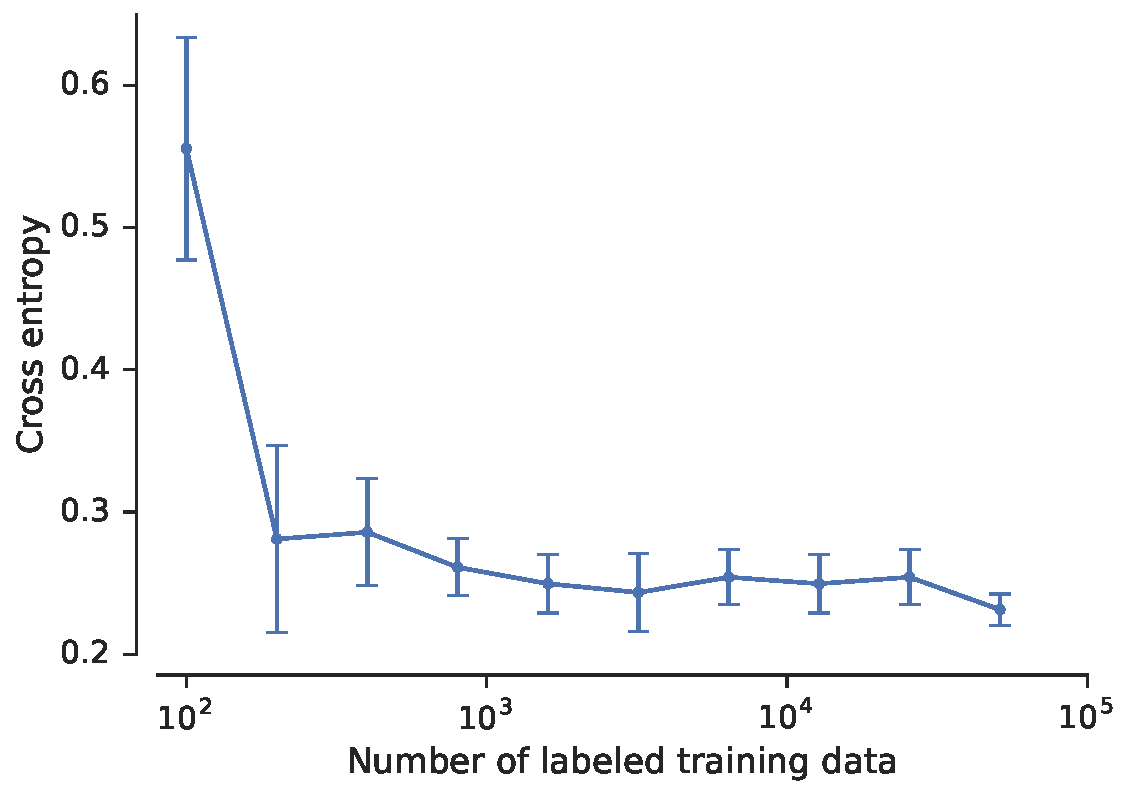
\includegraphics[width=\columnwidth]{figures/loss_vs_n.pdf}
  \caption{Cross-entropy as a function of the number of labeled examples in the training set.}
  \label{fig:loss_vs_n}
\end{figure}

\begin{figure}
  \centering
  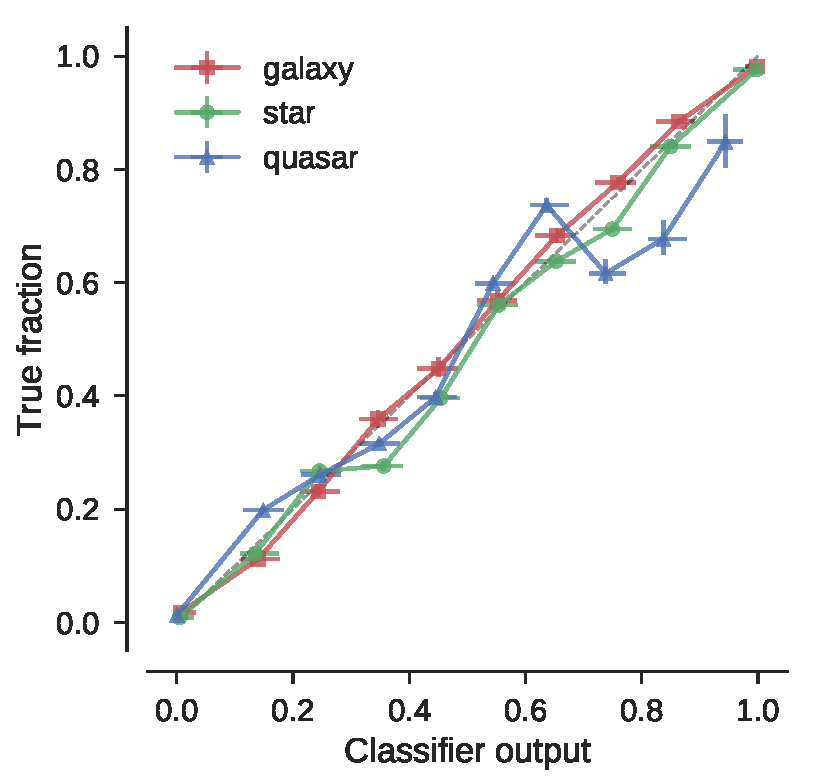
\includegraphics[width=\columnwidth]{figures/calibration_curve.pdf}
  \caption{
    Calibrations curve for galaxies (red), stars(green), and quasars (blue).
    We compare the true fraction to the probabilistic output generated by the classifier for each type
    of objects.
    The dashed line displays the ideal relationship.
    The $1 \sigma$ error bars are computed following \citet{paterno2004calculating}.}
  \label{fig:calibration_curve}
\end{figure}


\begin{figure}
  \centering
  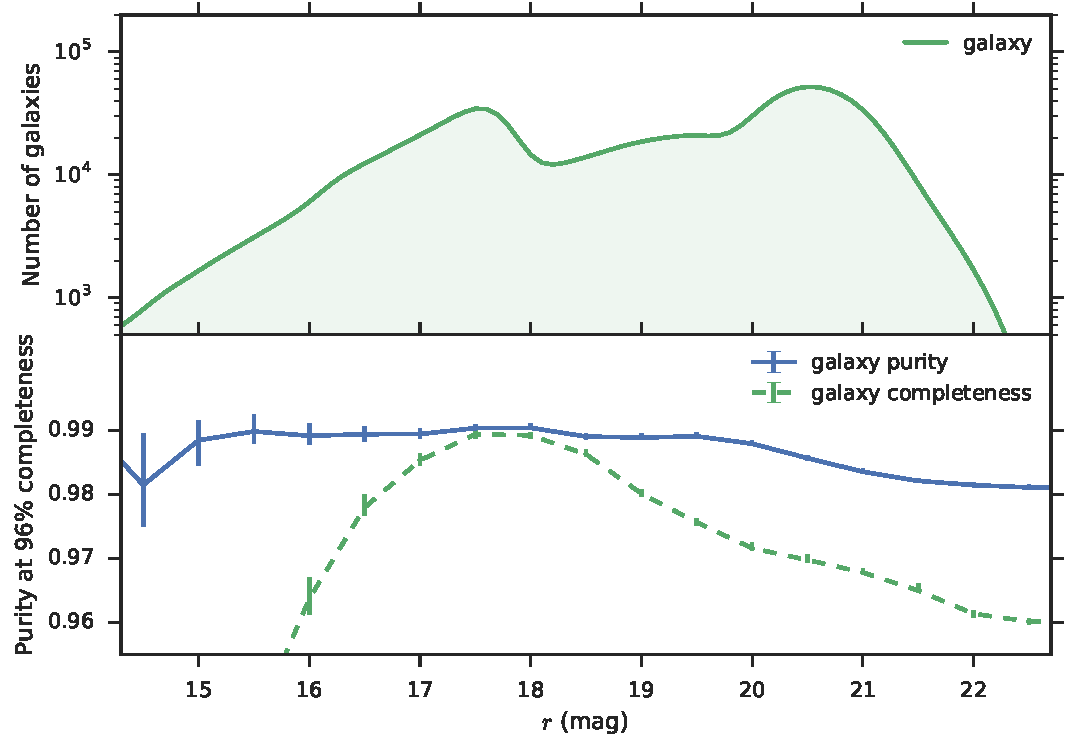
\includegraphics[width=\columnwidth]{figures/gal_comp_pur.pdf}
  \caption{
    Galaxy completeness and purity values as functions of the $r$-band magnitude.
    The upper panel shows the differential counts for true galaxies in the test set.
    The lower panel shows the galaxy completeness and purity for the integrated counts.
    We use the threshold value of 0.826 to obtain overall completeness of $96\%$.
    The $1 \sigma$ error bars are calculated with a Bayesian method in
    \citet{paterno2004calculating}.}
  \label{fig:gal_comp_pur}
\end{figure}

\begin{figure}
  \centering
  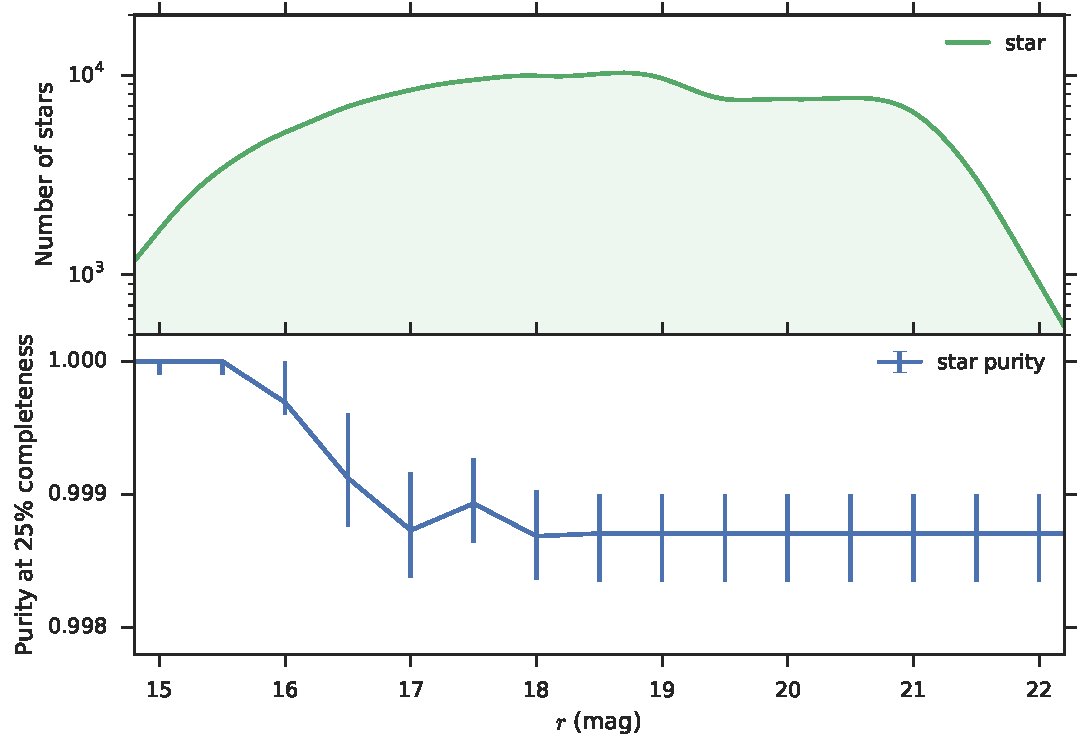
\includegraphics[width=\columnwidth]{figures/star_comp_pur.pdf}
  \caption{
    Similar to Figure \ref{fig:gal_comp_pur} but showing completeness for stars.
    We use the threshold value of 0.977 to obtain overall completeness of $25\%$.
    }
  \label{fig:star_comp_pur}
\end{figure}

\begin{figure}
  \centering
  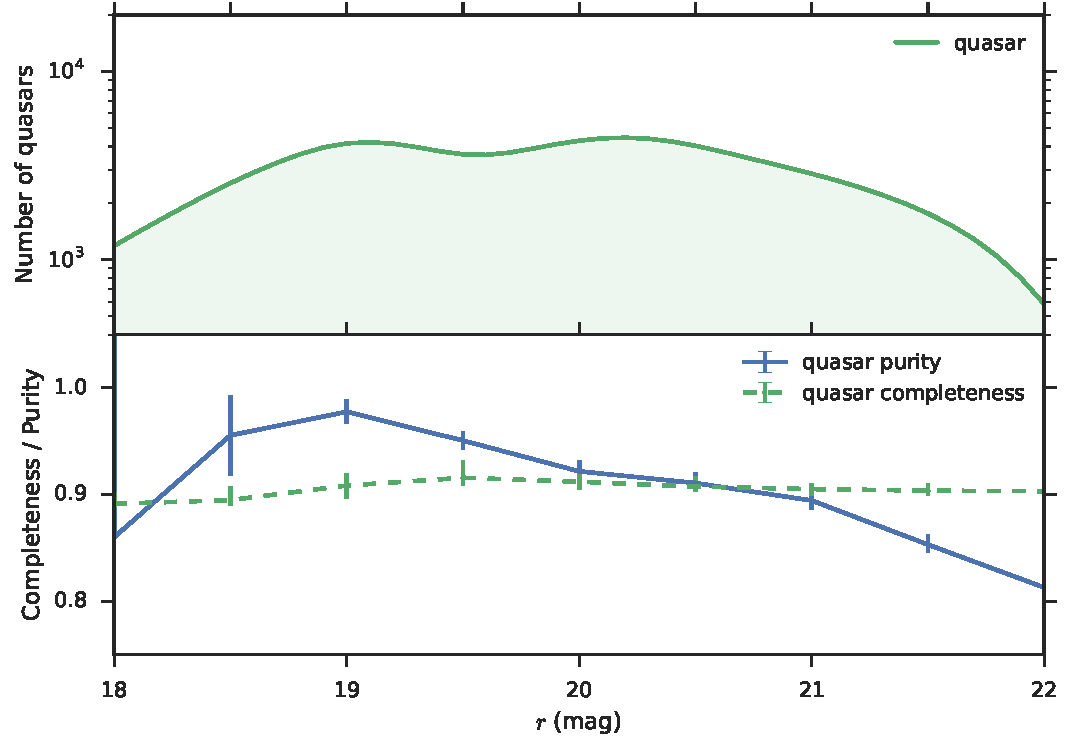
\includegraphics[width=\columnwidth]{figures/qso_comp_pur.pdf}
  \caption{
    Similar to Figure \ref{fig:gal_comp_pur} but showing completeness and purity for quasars.
    We use the threshold value of 0.541 to maximize $\sqrt{ c_q^2 + p_q^2 }$.
    }
  \label{fig:qso_comp_pur}
\end{figure}

Although our GAN generator is able to learn the original distribution of pixel intensities,
our main focus is on semi-supervised classification performance.
We perform semi-supervised training with a small random subset of the spectroscopic sample,
and the remaining training images are drawn from the photometric sample.
We perform eightfold cross-validation on the labeled training data to evaluate the cross-entropy
\citep[also called log loss;][]{murphy2012machine},
and the model that minimizes the cross-validation error is chosen as the best model.
Here, the cross-entropy is defined as
\begin{equation}
H = - \frac{1}{N} \sum_{i=0}^{N-1} \sum_{k=0}^{K-1} y_{i,k} \log \hat{y}_{i,k},
\end{equation}
where $y_{i,k}$ is the true labels (\ie $y_{i,k} = 1$ if sample $i$ has label $k$) and
$\hat{y}_{i,k}$ is the probability prediction made by the models.
Our final model is then applied to the blind test set, where we compare the model predictions with spectroscopic labels.
Figure \ref{fig:loss_vs_n} shows the cross-entropy as a function of the number of labeled examples.
As expected, we get better performance as we increase the number of labeled data,
but most of the improvement in performance comes from the first $1 \times 10^3$ labeled examples.
Thus, we use 1,024 labeled examples in the following sections.

Our GAN classifier is a probabilistic classifier, and its softmax function outputs a multiclass categorical
probability distribution.
Ideally, the probability distribution would be used in subsequent scientific analyses.
For example, we can in principle remove the contamination effect of stars when measuring auto-correlation functions of
luminous galaxies by weighting each object by the probability that it is a galaxy \citep{ross2011ameliorating}.
Thus, the probability estimates for each class should reflect the proportion of objects that actually belong to that class.
In Figure \ref{fig:calibration_curve}, we show the calibration curve \citep[or reliability curves;][]{degroot1983comparison},
where we bin the probability estimates and plot the true fraction of positive examples versus the probabilities assigned
by the classifier.
The calibration curve for galaxies is nearly diagonal and well-calibrated, so we can confidently use the
classifier output to estimate the probability that an object is a galaxy.
The calibration curve for stars is also nearly diagonal and well-calibrated,
while the probabilities assigned to quasars are not as accurate as stars or galaxies.
This might be due to the relatively small number of quasars in the training set.
Furthermore, quasars appear as point sources in photometry, rather than extended sources like galaxies,
and photometric images of quasars often have one or more saturated pixels.
The GAN classifier's over-reliance on morphological features would worsen the classification performance for quasars.

Probability estimates can also be converted into discrete class labels by choosing a probability threshold.
A naive way is to choose the most probable class label as the final classification.
However, this simple approach is not optimal in cases where there is class imbalance,
certain science requirements have to be satisfied, or misclassifying one class is more costly than misclassifying the others.
Thus, it is ideal to adjust the classification decision threshold by considering the model's operating conditions
For example, the optimal optimal star-galaxy catalog for fast-transient surveys would produce a pristine sample of point sources, and
\citet{miller2017preparing} adjust the threshold to identify as many point sources as possible, while minimizing the number
of galaxies misclassified as stars.
In this paper, we follow our previous work \citep{kim2015hybrid}, and adopt the weak lensing science requirements of the DES
as a realistic operating condition.
The weak lensing science measurements of the DES require $c_g > 0.960$ and $p_g > 0.778$ to control the statistical and systematic errors
on the cosmological parameters, and $c_s > 0.250$ and $p_s > 0.970$ for stellar Point Spread Function (PSF) calibration
\citep{soumagnac2013star}.
Although other surveys, such as SDSS or LSST, will likley have different science requirements,
we adopt these values,
and compute the galaxy purity at $96\%$ completeness and the star purity at $25\%$ completeness.
Here, we define the galaxy completeness $c_g$ as the number of true galaxies classified as galaxies
compared to the total number of galaxies in the whole sample:
\begin{equation}
c_g = \frac{ N_g }{ N_g + M_g },
\end{equation}
where $N_g$ is the number of true galaxies classified as galaxies, and
$M_g$ is the number of true galaxies classified as stars or quasars.
The galaxy purity $p_g$ is defined as the fraction of true galaxies among objects that are classified as galaxies:
\begin{equation}
p_g = \frac{ N_g }{ N_g + M_s + M_q },
\end{equation}
where $M_s$ is the number of true stars classified as galaxies,
and $M_q$ is the number of true quasars classified as galaxies.
We define the completeness and purity for stars and quasars in a similar way.

In Figure \ref{fig:gal_comp_pur}, we show the galaxy completeness and purity values as a function of apparent magnitude
in the $r$ band.
For galaxies, the overall purity is $98.1\%$ at $96.0\%$ completeness.
Comparing these values to the results of our previous work \citep{kim2017star},
where a supervised method using convolutional neural networks
was shown to achieve a purity of $99.1\%$ at $96.0\%$ completeness on the SDSS data, our semi-supervised approach
performs slightly worse than the state-of-the-art supervised algorithm on the spectroscopic sample.
However, it is highly likely that supervised algorithms, which are
trained on the spectroscopic sample, will show worse performance when they are applied on the photometric sample,
since we are extrapolating our models beyond the limits of training data.
In contrast, since our semi-supervised algorithm is trained on the photometric sample, we are
extrapolating beyond the limits of underlying data distribution when we measure its performance on
the spectroscopic sample.
Thus, when our semi-supervised approach is applied to the photometric sample, its performance will likely be
competitive to that of supervised algorithms, and it may even significantly outperform supervised learning
on the SDSS photometric sample.

In Figure \ref{fig:star_comp_pur}, we show the star purity as a function of $r$-band magnitude.
For stars, the overall purity is $99.9\%$ at $25.0\%$ completeness.
To choose the threshold for assigning quasar classifications, we maximize the metric $\sqrt{ c_q^2 + p_q^2 }$.
We show the completeness and purity values for quasars in Figure \ref{fig:qso_comp_pur}.
The overall purity of the quasars is rather low at $80.6\%$ but the completeness $90.3\%$.
Figure \ref{fig:qso_comp_pur} shows that the low purity is due to quasars at $r \ga 20.5$,
where counts reach their peak.
The low value may also be due to the fact that there are relatively small number of training examples for quasars.


\subsection{Uncertainty}

\begin{figure}
  \centering
  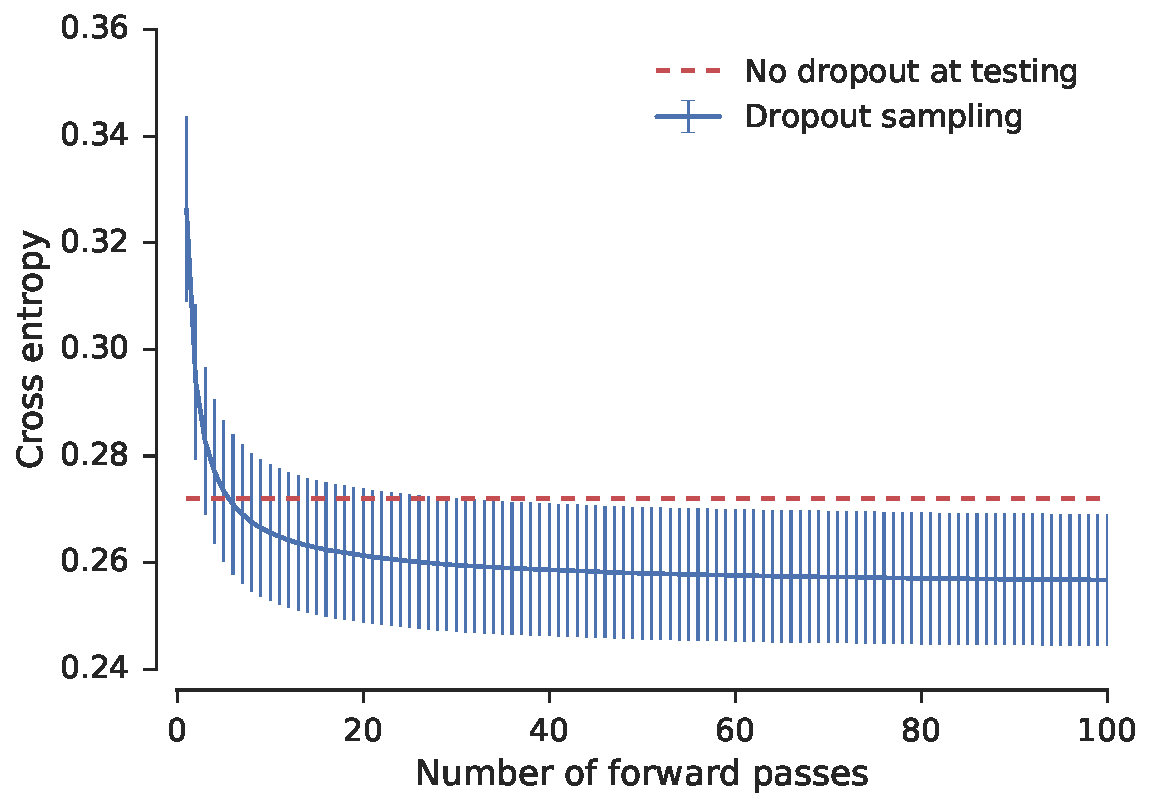
\includegraphics[width=\columnwidth]{figures/mcmc_loss.pdf}
  \caption{
    Cross-entropy for different numbers of averaged forward passes in dropout sampling.
    The solid blue line indicates mean cross-entropy of 10 experiments, and the error bars are 1 standard deviation.
    The red dotted line shows the cross-entropy with no dropout at testing time.
    }
  \label{fig:mcmc_loss}
\end{figure}

\begin{figure}
  \centering
  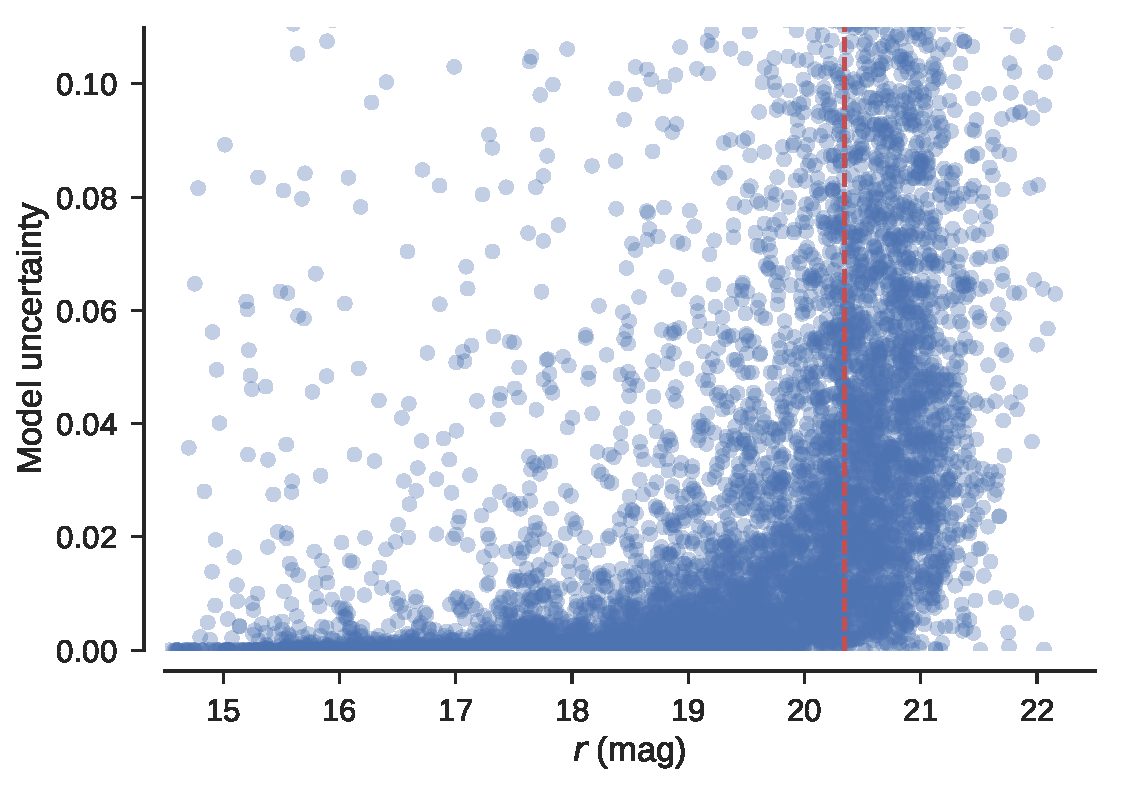
\includegraphics[width=\columnwidth]{figures/uncertainty_vs_mag.pdf}
  \caption{
    Model uncertainty as a function of $r$-band magnitude for 10,000 randomly selected objects in the test set.
    Model uncertainty is measured by the standard deviation of 100 forward passes in dropout sampling.
    }
  \label{fig:uncertainty_vs_mag}
\end{figure}

As mentioned in Section \ref{sec:dropout_sampling}, although many deep neural network architectures are trained with dropout,
it is usually not used at testing time.
In Figure \ref{fig:mcmc_loss}, we show the cross-entropy on the test set as a function of the number of forward passes
used in dropout sampling.
When we use dropout for only a few forward passes, the performance is worse than the deterministic case where all neurons are activated.
However, by performing multiple forward passes with dropout and averaging the results, we reduce the cross-entropy by more than one
standard deviation after 30 samples.
Thus, we can improve our predictive performance significantly by using dropout sampling, although this adds some computational cost
at testing time.
Furthermore, dropout sampling enables us to estimate model uncertainty, which could be an important source of systematic error
if the probability estimates are used in subsequent scientific analyses \citep{ross2011ameliorating}.
Figure \ref{fig:uncertainty_vs_mag} shows the standard deviation of 100 different probability estimates from dropout sampling
as a function of $r$-band magnitude.
The model uncertainties are relatively small at bright magnitudes $r \la 20$, but our model produces increasingly uncertain
probability estimates for faint objects as it becomes difficult to distinguish between noise and faint sources.

% Conclusions
\section{Conclusions}
  \label{sec:conclusions}

We have presented a semi-supervised generative adversarial network for classifying stars and galaxies in the SDSS photometric images.
We have demonstrated that the brightness and size distributions of images generated by our generative model
are in good agreement with those of the SDSS photometric images.
However, unlike most work on GANs, our focus was not solely on the generation of realistic images.
By using a small number of labeled images in conjunction with a large amount of unlabeled training data,
we have shown that our semi-supervised GAN is able to provide a classification that is comparable to the state-of-the-art
supervised methods.

Our goal in this work was not to obtain the best classification performance for the SDSS,
but to explore the potential impact of semi-supervised learning in the next generation of photometric surveys, such as DES and LSST.
As future surveys probe larger and larger cosmological volumes, it is not clear if we will have sufficient spectroscopic observations
for supervised learning algorithms.
Even with the scale of expansive spectroscopic coverage of the original SDSS and the Baryon Oscillation Spectroscopic Survey
\citep[BOSS;][]{dawson2012baryon}, the spectroscopic sample will be susceptible to selection bias,
and a truly unbiased training set will have only a minimal number of examples.
Thus, semi-supervised and unsupervised learning will become increasingly important in future surveys.
To emulate this scenario, we have performed most of our analysis using only $10^3$ spectroscopic labels, and
found that the classification performance is competitive with supervised algorithms.

In this work, we have also demonstrated the use of various scientific tools to validate our deep generative model.
In astronomy, we have powerful techniques for characterizing classifications, even in the absence of spectroscopic labels.
In contrast, most of the data sets used in the deep learning community are composed of natural images and text corpuses,
which lack such statistical techniques,
and direct comparison between different generative models is often difficult 
\citep{theis2016note}.
As a result, Astronomy has the potential to provide frameworks for evaluation and interpretation of generative models.

In this paper, we used photometry and spectra from the SDSS.
While the SDSS provides a rich data set for deep learning,
it is limited to the optical and near-infrared wavelengths.
We plan to combine multiple photometry sources by matching the SDSS objects to
photometric objects in other surveys, such as GALEX, WISE, or UKIDSS.
We are also exploring different strategies to improve the quality of generated images.
For example, although we used feature matching in this work to obtain a strong classifier,
if the goal is to improve the quality of generated images, an alternative technique
called minibatch discrimination will likely work better \citep{salimans2016improved,dai2017good}.
Finally, future studies could investigate the application of deep generative models in other settings,
such as unsupervised classification, object segmentation, and redshift estimation.

\section*{Acknowledgements}

We acknowledge support from the National Science Foundation Grant AST-1313415.

This work used the Extreme Science and Engineering Discovery Environment (XSEDE), which is supported by National Science Foundation grant number ACI-1548562.

Funding for the Sloan Digital Sky Survey IV has been provided by
the Alfred P. Sloan Foundation, the U.S. Department of Energy Office of
Science, and the Participating Institutions. SDSS-IV acknowledges
support and resources from the Center for High-Performance Computing at
the University of Utah. The SDSS web site is \url{http://www.sdss.org/}.

\bibliographystyle{mnras}
\bibliography{main}

% Don't change these lines
\bsp	% typesetting comment
\label{lastpage}
\end{document}

% End of mnras_template.tex
